\documentclass[11pt, oneside]{article} 
\usepackage{geometry}
\geometry{letterpaper} 
\usepackage{graphicx}
	
\usepackage{amssymb}
\usepackage{amsmath}
\usepackage{parskip}
\usepackage{color}
\usepackage{hyperref}

\graphicspath{{/Users/telliott_admin/Dropbox/Tex/png/}}
% \begin{center} \includegraphics [scale=0.4] {gauss3.png} \end{center}

\title{Generators, logarithms, inverses}
\date{}

\begin{document}
\maketitle

\large

\url{http://www.cs.utsa.edu/~wagner/laws/FFM.html}

\subsection*{Improved multiplication, and generators for GF(2e8)}
Following the reference, we first take another look at multiplication.

Previously, we multiplied \textbf{0xb6 * 0x53} by doing $(7,5,4,2,1) *  (6,4,1,0)$
\begin{center} 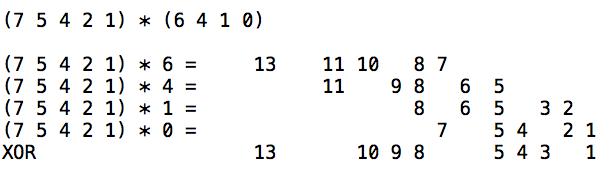
\includegraphics [scale=0.5] {figs/GFmath1.png} \end{center}

followed by the modulus operation by repeated $\oplus$ at the end:
\begin{center} 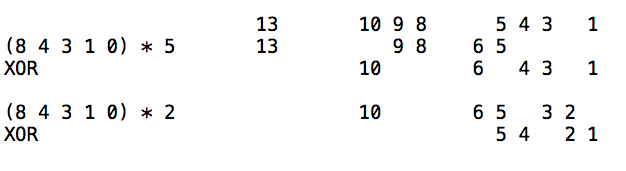
\includegraphics [scale=0.5] {figs/GFmath2.png} \end{center}

The following is given as a more efficient version.  Whenever a value in the program exceeds 255, we do an XOR with the irreducible polynomial.

Again we have $(7,5,4,2,1) *  (6,4,1,0)$.  In the first phase (round 0) we have just $(7,5,4,2,1) * 0$.  In the round 1 we multiply by $1$ (i.e. $x$) to give $(8,6,5,3,2)$, which we immediately XOR with the special polynomial $m(x) = (8,4,3,1,0)$, and then XOR that with what we had from phase 0.

\begin{center} 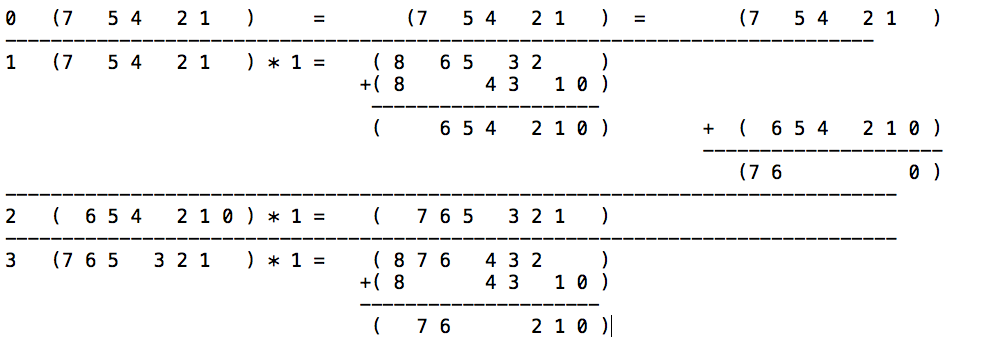
\includegraphics [scale=0.5] {figs/GFmath6.png} \end{center}
In round 2 we bump up the multiplicand by a factor of 2 again (of course, it was reduced by the modulus in the previous round).  We do the same again in round 3, and find we have again exceeded the modulus.  So we do another XOR.

\begin{center} 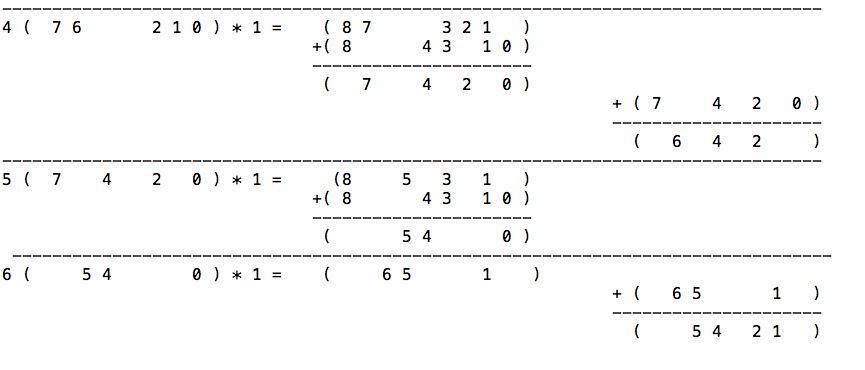
\includegraphics [scale=0.55] {figs/GFmath7.png} \end{center}
In round 4, we increase by a factor of 2, divide by the special number, and XOR what we accumulated before.  In round 6, we increase by a factor of 2 and do the modulus thing,  In round 6, we increase by 2-fold and do the XOR thing.  The result is $(5,4,2,1)$, which is the same as what we got before.

\subsection*{Generators in fields}
According to the reference a
\begin{quote}
A generator is an element whose successive powers take on every element except the zero.
\end{quote}
 Having faith that one exists we try various possibilities for $Z_{13}$:  powers of 5
 \[ 5 \]
 \[ 5^2 = 25 \mod 13 = 12 \]
 \[ 5^3 = 5 \times 12 \mod 13 = 8 \]
 \[ 5^4 = 5 \times 8 = 40 \mod 13 = 1 \]
 So now the pattern will repeat, and we have only 4 values.
 
 You could try 4
 \[ 4 \]
 \[ 4^2 = 16 \mod 13 = 3 \]
 \[ 4^3 = 4 \times 3 = 12 \mod 13 = 12 \]
 \[ 4^4 = 4 \times 12 = 48 \mod 13 = 9 \]
 \[ 4^5 = 4 \times 9 = 45 \mod 13 = 6 \]
 \[ 4^6 = 4 \times 6 = 24 \mod 13 = 9 \]
 \[ 4^7 = 4 \times 9 = 36 \mod 13 = 10 \]
 \[ 4^8 = 4 \times 10 = 40 \mod 13 = 1 \]
 so we terminate with only  8 values. 
 
 Persevere!  
 \[ 2 \times 1 = 2 \]
 \[ 2 \times 2 = 4 \]
 \[ 2 \times 3 = 8 \]
 \[ 2 \times 4 = 16 \mod 13 = 3 \]
 \[ 2 \times 3 = 6 \]
 \[ 2 \times 6 = 12 \]
 \[ 2 \times 12 = 24 \mod 13 = 11 \]
 \[ 2 \times 11 = 22 \mod 13 = 9 \]
 \[ 2 \times 9 = 18 \mod 13 = 5 \]
 \[ 2 \times 5 = 10 \]
 \[ 2 \times 10 = 20  \mod 13 = 7 \]
 \[ 2 \times 7 = 14 \mod 13 = 1 \]
 
 We see that $2$ will generate:
 \[ 2,4,8,3,6,12,11,9,5,10,7,1 \]
 That is all the values we need.
 
 Generators are hard to discover.
 
 Here is an example from Kak, lecture 7.  Recall that the polynomials defined over $GF(2^3)$ modulo the irreducible polynomial $x^3 + x + 1$ consist of the finite set:
 
 \[ 0, \ \ \ 1, \ \ \ x, \ \ \ x + 1 \]
 \[ x^2, \ \ \ x^2 + 1, \ \ \ x^2 + x, \ \ \ x^2 + x + 1 \] 
 
 Kak says:
 
 \begin{quote}The generator g is that element which symbolically satisfies $g^3 + g + 1 = 0$, implying that such an element will obey $g^3 = -g - 1 = g + 1$\end{quote}.
 
The first element is $0$, then the generator gives us

\[ g^0 = 1 \]
\[ g^1 = g \]
\[ g^2 = g^2 \]
\[ g^3 = g + 1 \]
\[ g^4 = g(g^3) = g(g + 1) = g^2 + g \]
\[ g^5 = g(g^4) = g(g^2 + g) = g^3 + g^2 = g^2 + g + 1 \]
\[ g^6 = g(g^5) = g(g^2 + g + 1) = g^3 + g^2 + g = g^2 + 1 \]
\[ g^7 = g(g^6) = g(g^2 + 1) = g^3 + g = 1 \]

Kak again:

\begin{quote}
Since every polynomial in $GF(2^n)$ is represented by a power of $g$, multiplying any two polynomials in $GF(2^n)$ becomes trivial — we just have to add the exponents of $g$ modulo $(2^n$ minus $1)$. ..
using the generator notation allows the multiplications of the elements of the finite field to be carried out without reference to the irreducible polynomial.\end{quote}
 
 \subsection*{Generator for GF(2e8)}
 
 For $GF(2^8)$, \textbf{0x03} $ = 3$ is a generator.

\textbf{0x03 * 0x03 = 0011 * 0011 = 0110 $\oplus$ 0011 = 0101 = 0x05}

\textbf{0x03 * 0x05  =  1010 $\oplus$ 0101 = 1111 = 0x0f }

\textbf{0x03 * 0x0f  =  0000 \ 1111 $\oplus$ 0001 \ 1110 = 0001 \ 0001 = 0x11 }

\textbf{0x03 * 0x11  = 0010 \ 0010 $\oplus$ 0001 \ 0001 = 0011 \ 0011 = 0x33 }

\textbf{0x03 * 0x33  = 0110 \ 0110 $\oplus$ 0011 \ 0011 = 0101 \ 0101 = 0x55 }

\textbf{0x55 * 0x11  = 1010 \ 1010 $\oplus$ 0101 \ 0101 = 1111 \ 1111 = 0xff }

The next step is the first one to involve the modulus:  The first term is the shifted \textbf{0xff}.

\textbf{0x03 * 0x11  = 1 \ 1111 \ 1110 $\oplus$ 1 \ 0001 \ 1011 = 1110 \ 0101}

\hspace{7em} \textbf{1110 \ 0101 $\oplus$ 1111 \ 1111 = 0001 1010 =  0x1a }

Another way to do the last step
\[ 255 * 2 = 510, \ \  \mod 256 = 254, \ \  \oplus \ 27 = 229, \ \  \oplus \ 255 = 26 \]


Here is part of it.  Somehow it comes around.

\begin{center} 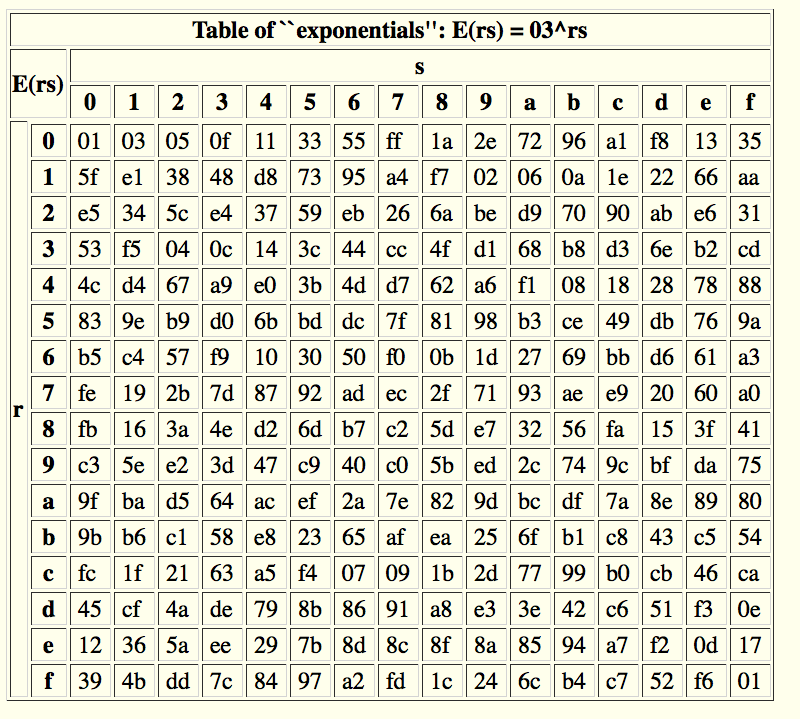
\includegraphics [scale=0.5] {figs/wagner4.png} \end{center}

There is a hard way and an easy way to use the table.  The hard way is the following.  Let's check the multiplication we did before:  \textbf{0xb6 $\times$ 0x53}.  The answer was \textbf{0x36}.  

Scour through the table to find the entry that is equal to \textbf{0xb6} and find it indexed as the power \textbf{0xb1}.  Similarly look up \textbf{0x53}, we find it indexed as the power \textbf{0x30}.

Multiply by adding the powers:  \textbf{0xb1} + \textbf{0x30} = \textbf{0xe1} (Do the addition modulo 256 if necessary).  Index into the table by the power \textbf{0xe1} and find \textbf{0x36} .  That's the same answer we got before.

The easy way, of course, is to make another table, of logarithms.  Take every pair \textbf{index, value} from the table of exponentials that we have, and switch it so the value becomes a new index and the index a new value.  Use the new index and value to construct the table of logarithms. Just do the lookup for the first part of the method in the logarithms table.

\subsection*{multiplicative inverse}

As I mentioned in the previous chapter, I used Kak's method to find all 65536 possible products of the numbers in the field $GF(2^8)$.  In the process I verified that for any product $p$ (except 0) and any factor $a$ there exists one and only one $b$ such that $a \times b = p$.  

This is also true for $p = 1$.  Every number has a multiplicative inverse.

If two numbers produce $p = 1$ when they are multiplied together, then their powers must add to give 255.  (0 is not generated as any power of the generator, the list of powers repeats after 255 values).

If we look in the table of logarithms for \textbf{0x53} we find \textbf{0x30}, and if we look for \textbf{0xca} and find \textbf{0xcf}.  Add them to obtain \textbf{0x30 + 0xcf = 0xff}.  Look in the table of exponentials and see the \textbf{0xff} indeed corresponds to \textbf{0x01}.



\end{document}